\documentclass[conference]{IEEEtran}
% *** GRAPHICS RELATED PACKAGES ***
%
\ifCLASSINFOpdf
  \usepackage[pdftex]{graphicx}
  % declare the path(s) where your graphic files are
  % \graphicspath{{../pdf/}{../jpeg/}}
  % and their extensions so you won't have to specify these with
  % every instance of \includegraphics
  \DeclareGraphicsExtensions{.pdf,.jpeg,.png}
\else
  % or other class option (dvipsone, dvipdf, if not using dvips). graphicx
  % will default to the driver specified in the system graphics.cfg if no
  % driver is specified.
  \usepackage[dvips]{graphicx}
  % declare the path(s) where your graphic files are
  % \graphicspath{{../eps/}}
  % and their extensions so you won't have to specify these with
  % every instance of \includegraphics
  % \DeclareGraphicsExtensions{.eps}
\fi

\usepackage{pgf}
%\usepackage{tikz}
%\usetikzlibrary{arrows,automata}

\definecolor{darkgreen}{rgb}{0,0.7,0}

\newif\ifdraft
\drafttrue
%\draftfalse
\ifdraft
 \newcommand{\katznote}[1]{ {\textcolor{blue} { ***Dan:   #1 }}}
 \newcommand{\ketanote}[1]{{\textcolor{orange}  { ***Ketan:   #1 }}}
 \newcommand{\kriedernote}[1]{ {\textcolor{darkgreen}  { ***Scott:   #1 }}}
 \newcommand{\note}[1]{ {\textcolor{red}    {\bf #1 }}}
\else
 \newcommand{\katznote}[1]{}
 \newcommand{\kriedernote}[1]{}
 \newcommand{\note}[1]{}
\fi
% correct bad hyphenation here
%\hyphenation{op-tical net-works semi-conduc-tor}

\hyphenation{Queuing}

\begin{document}
%
% can use linebreaks \\ within to get better formatting as desired
\title{Statement of Research}

%\author{\IEEEauthorblockN{Auth1\IEEEauthorrefmark{1},
%Auth2\IEEEauthorrefmark{1}\IEEEauthorrefmark{1}, 
%Auth3\IEEEauthorrefmark{1},
%\IEEEauthorblockA{\IEEEauthorrefmark{1}Argonne National Laboratory}
%}}

\author{Scott J. Krieder, 3rd Year Doctoral Student\\
Department of Computer Science, Illinois Institute of Technology}

\maketitle


\IEEEpeerreviewmaketitle

\section{Funding History}
As a 3rd year PhD student I have been supported as both a Teaching and Research Assistant in the Department of Computer Science. As a Teaching Assistant, I have mentored students in multiple courses including: Computer Organization, Systems Programming, Operating Systems, Advanced Operating Systems, and Data-Intensive Computing. In addition, I am supported this calendar year by a 2013 Starr/Fieldhouse Fellowship \cite{Starr} from the Illinois Institute of Technology to pursue a collaboration with Argonne National Laboratory and the Computation Institute at the University of Chicago for my work titled ``Towards the Support for Many-Task Computing on Many-Core Computing Platforms''. \cite{kriederGCASR12}\cite{kriederXSEDE12}\cite{kriederSC12}\cite{grimmerEUROSYS13}

\section{Research Contributions}
Current software and hardware limitations prevent Many-Task Computing (MTC) workloads from leveraging hardware accelerators boasting Many Core Computing architectures. Current work aims to address the programmability gap between MTC and accelerators, through the innovative CUDA middleware GeMTC. By working at the warp level, GeMTC enables heterogeneous task scheduling and 10x number of workers compared to CUDA. In order to span multiple accelerators across nodes, this work has adopted the Swift parallel programming system \cite{zhao2007swift}, which can both support fine grained millisecond tasks and extreme scale supercomputers at 100K-cores. Currently CUDA developers may only have a maximum of 16 kernels running concurrently, one kernel per streaming multiprocessor (SM). The problem is that all kernels have to start and end at the same time, causing extreme inefficiencies in heterogeneous workloads. By working at the warp level and trading local memory for concurrency the GeMTC framework is able to run up to 84 concurrent kernels. \cite{kriederSC12} This middleware allows independent kernels (MIMD style) to be launched and managed on many-core architectures that traditionally only support SIMD. \cite{kriederXSEDE12} As shown in \ref{fig:big_pic} Swift/T \cite{wozniak13swift} makes calls to the GeMTC API and passes tasks into memory on the device. Warp workers pick up tasks from the in memory queue, execute the task with the given parameters and place results on an outgoing result queue. Finally, Swift/T will poll the device and return results from the result queue back to the appropriate task in the swift script. The worker count is dependent on hardware architectures, where current generation GPUs have O(10) Streaming Multiprocessors (SMX), O(100) Warps, and O(1000) cores. \cite{GK110}
\begin{figure}[h]
\centering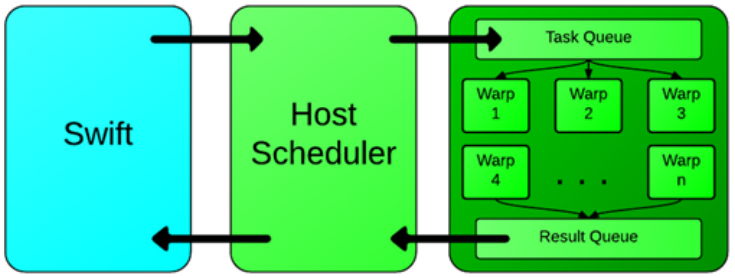
\includegraphics[width=8cm]{imgs/big_picture.png}
\caption{Flow of a task through Swift/T and GeMTC.}
\label{fig:big_pic}
\end{figure}

\section{Future Direction}
Current work designed and implemented the GeMTC framework. A sub-allocator provides improved memory management for dynamic tasks. Integration between GeMTC + Swift/T provides application support, data-flow parallelism, and multi-node scalability. Future work aims to abstract for additional accelerator support (Intel Xeon Phi, AMD GPUs), evaluate real applications such as the Open Protein Simulator (OOPS) \cite{OOPS}, and improve current framework performance.

\bibliographystyle{IEEEtran}
\bibliography{ref}
\end{document}
